%%%%%%%%%%%%%%%%%%%%%%%%%%%%%%%%%%%%%%%%%%%%%%%%%%%%%%%%%%%%%%%%%%%%%%%%%%%%
% AGUJournalTemplate.tex: this template file is for articles formatted with LaTeX
%
% This file includes commands and instructions
% given in the order necessary to produce a final output that will
% satisfy AGU requirements, including customized APA reference formatting.
%
% You may copy this file and give it your
% article name, and enter your text.
%
%
% Step 1: Set the \documentclass
%
% There are two options for article format:
%
% PLEASE USE THE DRAFT OPTION TO SUBMIT YOUR PAPERS.
% The draft option produces double spaced output.
%

%% To submit your paper:
\documentclass[draft]{agujournal2019}
\usepackage{url} %this package should fix any errors with URLs in refs.
\usepackage{lineno}
\linenumbers
%%%%%%%
% As of 2018 we recommend use of the TrackChanges package to mark revisions.
% The trackchanges package adds five new LaTeX commands:
%
%  \note[editor]{The note}
%  \annote[editor]{Text to annotate}{The note}
%  \add[editor]{Text to add}
%  \remove[editor]{Text to remove}
%  \change[editor]{Text to remove}{Text to add}
%
% complete documentation is here: http://trackchanges.sourceforge.net/
%%%%%%%

\draftfalse

%% Enter journal name below.
%% Choose from this list of Journals:
%
% JGR: Atmospheres
% JGR: Biogeosciences
% JGR: Earth Surface
% JGR: Oceans
% JGR: Planets
% JGR: Solid Earth
% JGR: Space Physics
% Global Biogeochemical Cycles
% Geophysical Research Letters
% Paleoceanography and Paleoclimatology
% Radio Science
% Reviews of Geophysics
% Tectonics
% Space Weather
% Water Resources Research
% Geochemistry, Geophysics, Geosystems
% Journal of Advances in Modeling Earth Systems (JAMES)
% Earth's Future
% Earth and Space Science
% Geohealth
%
% ie, \journalname{Water Resources Research}

\journalname{Geophysical Research Letters}


\begin{document}

%% ------------------------------------------------------------------------ %%
%  Title
%
% (A title should be specific, informative, and brief. Use
% abbreviations only if they are defined in the abstract. Titles that
% start with general keywords then specific terms are optimized in
% searches)
%
%% ------------------------------------------------------------------------ %%

% Example: \title{This is a test title}

\title{Depth of the source of the tectonic tremor in the eastern Olympic Peninsula, Washington}

%% ------------------------------------------------------------------------ %%
%
%  AUTHORS AND AFFILIATIONS
%
%% ------------------------------------------------------------------------ %%

% Authors are individuals who have significantly contributed to the
% research and preparation of the article. Group authors are allowed, if
% each author in the group is separately identified in an appendix.)

% List authors by first name or initial followed by last name and
% separated by commas. Use \affil{} to number affiliations, and
% \thanks{} for author notes.
% Additional author notes should be indicated with \thanks{} (for
% example, for current addresses).

% Example: \authors{A. B. Author\affil{1}\thanks{Current address, Antartica}, B. C. Author\affil{2,3}, and D. E.
% Author\affil{3,4}\thanks{Also funded by Monsanto.}}

\authors{Ariane Ducellier\affil{1}}


% \affiliation{1}{First Affiliation}
% \affiliation{2}{Second Affiliation}
% \affiliation{3}{Third Affiliation}
% \affiliation{4}{Fourth Affiliation}

\affiliation{1}{University of Washington}
%(repeat as many times as is necessary)

%% Corresponding Author:
% Corresponding author mailing address and e-mail address:

% (include name and email addresses of the corresponding author.  More
% than one corresponding author is allowed in this LaTeX file and for
% publication; but only one corresponding author is allowed in our
% editorial system.)

% Example: \correspondingauthor{First and Last Name}{email@address.edu}

\correspondingauthor{Ariane Ducellier}{ducela@uw.edu}

%% Keypoints, final entry on title page.

%  List up to three key points (at least one is required)
%  Key Points summarize the main points and conclusions of the article
%  Each must be 100 characters or less with no special characters or punctuation and must be complete sentences

% Example:
% \begin{keypoints}
% \item	List up to three key points (at least one is required)
% \item	Key Points summarize the main points and conclusions of the article
% \item	Each must be 100 characters or less with no special characters or punctuation and must be complete sentences
% \end{keypoints}

\begin{keypoints}
\item enter point 1 here
\item enter point 2 here
\item enter point 3 here
\end{keypoints}

%% ------------------------------------------------------------------------ %%
%
%  ABSTRACT
%
% A good abstract will begin with a short description of the problem
% being addressed, briefly describe the new data or analyses, then
% briefly states the main conclusion(s) and how they are supported and
% uncertainties.
%% ------------------------------------------------------------------------ %%

%% \begin{abstract} starts the second page

\begin{abstract}
enter abstract here

\end{abstract}



%% ------------------------------------------------------------------------ %%
%
%  TEXT
%
%% ------------------------------------------------------------------------ %%

%%% Suggested section heads:
% \section{Introduction}
%
% The main text should start with an introduction. Except for short
% manuscripts (such as comments and replies), the text should be divided
% into sections, each with its own heading.

% Headings should be sentence fragments and do not begin with a
% lowercase letter or number. Examples of good headings are:

% \section{Materials and Methods}
% Here is text on Materials and Methods.
%
% \subsection{A descriptive heading about methods}
% More about Methods.
%
% \section{Data} (Or section title might be a descriptive heading about data)
%
% \section{Results} (Or section title might be a descriptive heading about the
% results)
%
% \section{Conclusions}


\section{Introduction}
%Text here ===>>>

Tremor is a long (several seconds to many minutes), low amplitude seismic signal, with emergent onsets, and an absence of clear impulsive phases. Tectonic tremor have been explained as a swarm of small, low frequency earthquakes \cite{SHE_2007}, that is small magnitude earthquakes (M $\sim$ 1) which frequency content (1-10 Hz) is lower than for ordinary earthquakes (up to 20 Hz). The source of the low-frequency earthquakes is located on the plate boundary, and their focal mechanisms represent shear slip on a low-angle thrust fault dipping in the same direction as the plate interface \cite{IDE_2007}. Due to the lack of clear impulsive phases in the tremor signal, it is difficult to determine the depth of the tremor source with the same precision, and it is assumed to be also located close to the plate boundary. In subduction zones such as Nankai and Cascadia, tectonic tremor observations are spatially and temporally correlated with slow slip observations \cite{OBA_2002}; \cite{ROG_2003}. Due to this correlation, these paired phenomena have been called Episodic Tremor and Slip (ETS).

tremor have been explained by silica-rich fluid flow.

Specific question - Depth of the low-frequency earthquake on the plate boundary. More difficult for the tremor because no phase onset.

Explain here about the link between tremor and quartz vein. Problem: LFE on a plane / zone with quartz vein is several km thick. Interested in location and thickness of the tremor zone.

References on quartz veins

Audet and B\"urgmann (2014 ~\cite{AUD_2014}) studied the relationship between the ratio between P-wave velocity and S-wave velocity in the subducted oceanic crust and the forearc and the periodicity of slow earthquakes. They computed the $V_P / V_S$ ratio from receiver functions and data from the literature. They noticed that slow earthquakes are associated with a high $V_P / V_S$ ratio in the subducted oceanic crust, but without relationship with recurrence time. However, they pointed out that the recurrence time of slow earthquakes increases linearly with the $V_P / V_S$ ratio of the forearc. Moreover, along a margin-perpendicular profile from northern Cascadia, the $V_P / V_S$ ratio of the forearc, and the recurrence time of Episodic Tremor and Slip (ETS) events, decrease with increasing depth. The authors explained the low $V_P / V_S$ ratio in the forearc by the enrichment of forearc minerals in fluid-dissolved silica derived from the dehydration of the downgoing slab. However, they estimated that the fluid flux required for the formation of quartz veins was two orders of magnitude greater than the fluid production rates estimated from the dehydration of the slab.They hypothesized that silica-saturated fluids may originate from the complete serpentinization of the mantle near the wedge corner. They suggested that higher temperature and quartz content at depth may lead to faster dissolution - precipitation processes and more frequent slip events. Their model could also explain the global variation in recurrence time, with mafic silica-poor regions having longer ETS recurrence times that felsic silica-rich regions.

Hyndman \textit{et al.} (2015 ~\cite{HYN_2015}) investigated the processes that control the position of Episodic Tremor and Slip (ETS) in the Cascadia subduction zone. They noticed that the high temperatures in the young subducting oceanic plate, the geodetic data, and the recordings of coseismic subsidence in buried coastal marshes during past great earthquakes, all point out to a downdip limit of the seismogenic zone located offshore. The position of the slow slip and the tremor is well known, although the depths have some uncertainty. The slip may extend seaward of the tremor, but there is a clear separation between the seismogenic zone and the ETS zone, with the ETS zone being located about 70 km east of the downdip of the seismogenic zone, and the volcanic arc being located about 100 km east of the ETS zone. A previous study showed that the position of the subduction zone ETS does not coincide with a specific temperature or dehydration reaction. The authors pointed out that ETS has been related to high pore fluid pressures close to the plate boundary. They argued that the bending of the subducting plate at the ocean trench may introduce a large amount of water in the upper oceanic mantle, resulting in extensive serpentinization. Moreover, the serpentinization of the fore-arc mantle corner may increase its vertical impermeability, while keeping a high permeability parallel to the fault, thus channelling all the fluid updip in the subducting oceanic crust. The dehydration of the serpentinite from the upper oceanic mantle, and the focusing of rising fluids along the plate boundary should result in large amounts of fluids available at the fore-arc mantle corner. Additionally, there seems to be a good coincidence between the location of the fore-arc mantle corner, and the location of ETS. The authors then observed that the deep fore-arc crust has a very low Poisson's ratio (less than 0.22), and that the only mineral with a very low Poisson's ratio is quartz (about 0.1), which led them to conclude that there may be a significant amount of quartz (about 10 \% in volume) in the deep fore-arc crust above the fore-arc mantle. Moreover, as the solubility of silica increases with temperature, fluids generated at depth and rising up the subduction channel should be rich in silica. The authors concluded that there may be a relation between quartz veins formation in the deep fore-arc crust and ETS. However, several constraints as the magnitude and mechanism of the low-frequency earthquakes, and the vertical extent of the tremor should be explained.

+ See papers by Fagereng

Review of past methods.

\citeA{LAR_2009}) stacked seismograms over all stations of the array for each component, and for three arrays in Cascadia. They then computed the cross-correlation between the horizontal and the vertical component, and found a distinct and persistent peak at a positive lag time, corresponding to the time between P-wave and S-wave arrivals. Using a standard layered Earth model, and horizontal slowness estimated from array analysis, they computed the depths of the tremor sources. They located the sources near or at the plate interface, with a much better depth resolution than previous methods based on seismic signal envelopes, source scanning algorithm, or small-aperture arrays. They concluded that at least some of the tremor consisted in the repetition of low-frequency events as was the case in Shikoku. A drawback of the method was that it could be applied only to tremor located beneath an array, and coming from only one place for an extended period of time.
Part of the specific question - Just on the plate boundary or overlying layer and how thick the layer is?

If the source is on the plate boundary, you should have a constant time lag between P-wave and S-wave arrivals, and a peak in the cross correlation between the vertical component and the horizontal component.

Explain here why it is going to work (No problem with tremor streaks)

\section{Data}

The data were collected during the 2009-2010 Array of Arrays experiment. Eight small-aperture arrays were installed in the northeastern part of the Olympic Peninsula, Washington. The aperture of the arrays was about 1 km, and station spacing was a few hundred meters. The arrays were around 5 to 10 km apart from each other (Figure 1). Most of the arrays were installed for more than a year, between June 2009 to September 2010, and were able to record the main August 2010 ETS event. Some of the arrays were also recording during the August 2011 ETS event. \citeA{GHO_2012} used a multibeam-backprojection (MBBP) technique to detect and locate tremor. They bandpass filtered the seismic data between 5 and 9 Hz. They divided the data into one-minute-long sliding independent (no overlap) time windows. They performed beam forming in the frequency domain at each array to determine the slowness vectors, and backprojected the slownesses in the 3-D space to locate the source of the tremor for each time window. We thus have two catalogs of tremors. The first one is a catalog of 28902 one-minute-long time windows during which tremor was detected between June 20th 2009 and September 30th 2010. For each time window, we have the beginning time, the end time, and the location (latitude and longitude) of the source of the tremor. The second one is a catalog of 5600 one-minute-long time windows between August 10th 2011 and September 6th 2011.

\begin{figure}
\noindent\includegraphics[width=\textwidth, trim={0cm 2.5cm 0cm 9.5cm},clip]{figures/arrays_location.eps}
\caption{Map showing the location of the eight arrays (red dots) used in this study. Grey dots are the locations of the source of the tremor recorded by the arrays. Inset shows the study area with the box marking the area covered in the main map. Contour lines represent a model of the depth of the plate interface \cite{MCC_2006}.}
\label{pngfiguresample}
\end{figure}

\section{Method}

We took a 5 km by 5 km grid cell located not too far (less than 25 km) from a given array. We then took all the one-minute-long time windows when tremor was detected and the source of the tremor was located inside this cell. For each one-minute-long time window, we downloaded the seismic data for each seismic station of the array. Then, for each seismic station and each channel, we detrended the data, tapered the first and last 5 seconds of the data with a Hann window, removed the instrument response, bandpass filtered between 2 and 8 Hz, and resampled the data to 20 Hz. All these preprocessing operations were done with the Python package obspy. For each seismic station and each one-minute-long time window, we cross correlated the vertical component with the East-West horizontal component and the North-South horizontal component. Then, we stacked the cross correlation functions over all the seismic stations of the array. We experimented with a linear stack, a power stack, and a phase-weighted stack. Figure 2 shows an example of the cross correlation functions as function of time for the Big Skidder array for the 82 one-minute long time windows when tremor was detected in a 5 km by 5 km grid cell centered on the array. We can see that for about half of the tremor windows, there is a peak in the cross correlation at about 4.7 s. As the energy of the P-waves is expected to be higher on the vertical component, and the energy of the S-waves to be higher on the horizontal components, we assume that this peak corresponds to the time lag between the arrival a direct P-wave and a direct S-wave. We then stacked the cross correlation functions over all the one-minute-long time windows. Again, we experimented with a linear stack, a power stack, and a phase-weighted stack. We assume that the time of the maximum absolute value of the peak of the stack is the time lag between the arrival of the direct P-wave and the arrival of the direct S-wave. \\

Only about half of the cross correlation functions have a distinct peak that coincides with the peak in the stacked cross correlation. The other cross correlations functions show either a distinct peak at another time lag, or no clearly visible peak. This may be due either because the source of the tremor during the corresponding one-minute-long time window was mislocated, either because the signal-to-noise ratio is too low. To improve the signal-to-noise ratio of the peak in the stacked cross correlation, we divided the one-minute-long time windows into two clusters, the ones that match well the stacked cross correlation, and the ones that do not math it well. For each one-minute-long time window, we compute the maximum absolute value of the cross correlation, its value at time 0, the time at which we takes its maximum absolute value, and the ratio between the
amplitude of the cross correlation peak to the root mean square error of the cross correlation function. We do this for both the East-West component and the North-South component, Each one-minute-long time window is thus associated to eight values of quality criteria. We then classified each one-minute-long time window into two different clusters, based on the value of these criteria, using a k-means clustering algorithm (function sklearn.cluster.KMeans from the Python library SciKitLearn). For each cluster, we then stacked the cross correlation functions over all the one-minute-long time windows belonging to the cluster. Figure 3 shows the stacked cross correlation for each of the clusters compared to the original stacked cross correlation for all the one-minute-long time windows. The clustering has improved the amplitude of the peak for one of the clusters, and made the peak nearly disappear for the other cluster. \\

We did this analysis for grid cells located in a 50 km by 50 km area centered on each of the eight arrays. We thus have 121 * 8 = 968 values of the time lag between the arrival of the direct P-wave and the arrival of the direct S-wave. We first assumed that the source of the tremor is located on the plate boundary, and we took a 1D velocity model for the overriding continental crust with $V_P$ = 6.4 km/s and $V_S$ = 3.6 km/s, to compute the depth of the tremor source for each location. \textcolor{red}{Modify this part if we use a 3D velocity model.}

\section{Results}

The analysis we carried out above may not lead to a reliable value of the depth of the source of the tremor for all relative positions of the array and the tremor. First, some areas are badly covered, and only a few tremor or no tremor at all were recorded. We limit our analysis to grid cells were tremor has been recorded during at least \textcolor{red}{10 (to be modified?)} one-minute-longtime windows. Another problem is that we assumed that the location of the tremor source is fixed during the one-minute-long time window where we compute the cross correlation of the seismic signal. However, this is not exactly the case. Indeed, during an ETS event, rapid tremor streaks have been observed propagating in the up-dip and down-dip directions at velocities ranging on average between 30 and 110, and up to 200 km/h \cite{GHO_2010_G3}, which corresponds to a source displacement of 0.5, 1.8, and 3.3 km during one minute. If we denote $t_P$ the arrival time of the direct P-wave, and $t_S$ the arrival time of the direct S-wave, the time lag between the two phase arrivals is $t_{lag} = t_S - t_P$. During the one-minute time window where we compute the cross correlation, the displacement $dx$ of the tremor source along the plate boundary should corresponds to a time lag difference $dt_{lag}$ shorter than a quarter of the dominant period of the tremor signal $T$ = 0.3 s. We computed the time lag difference for a displacement of the source of 0.5, 1.8 and 3.3 km in the up-dip direction, for stations aligned along the strike and along the dip direction. We assume that the source was located at 35 km depth, and we look at the time arrivals of the seismic wave for stations located up to 20 km from the epicenter, in the strike or the dip direction. The difference in time lags stays low for all the stations aligned along the strike of the plate boundary, even for tremor streaks traveling at 200 km/h. However, for the stations aligned along the dip of the plate boundary, the tremor streaks traveling at 200 km/h will cause a problem for the stations that are not immediately above the tremor source. The tremor streaks traveling at 110 km/h will cause a problem for the stations located more than 6 km updip of the tremor source. \\

\textcolor{red}{Something about how we choose the values we are keeping.} \\

\textcolor{red}{Something about interpolating the values of the different arrays.} \\

\textcolor{red}{Include here Figure 4 of the distance to the plate boundary + include values for the LFE families.} \\

\section{Discussion}

In the above part, we assumed that all the tremor within a given grid cell originate from the same depth, and we averaged over all the data to get the depth of the tremor source. However, instead of being located on the same plane near the plate boundary, the tremor may be scattered over a layer surrounding the plate boundary. To compute the thickness of this layer, we compute for each one-minute-long time window for which the cross correlation function matches well the stacked cross correlation the time lag between the time corresponding to the maximum absolute value for the cross correlation function and the time corresponding to the maximum absolute value for the stacked cross correlation. We then compute the standard deviation of this time lag, and compute the corresponding difference in depth using the 1D velocity model that we used previously.   \textcolor{red}{Something about computation of robust standard deviation.} We thus get the thickness of the layer from which the tremor originate. We used the same interpolation method as above to get the thickness of the layer for all the area covered by the eight arrays. Figure 5 shows the map of the thickness. \\

\textcolor{red}{Some interpretation.}

\section{Conclusion}

How analysis addresses the part of the specific question

How analysis addresses the specific question

How analysis addresses the general question



%%

%  Numbered lines in equations:
%  To add line numbers to lines in equations,
%  \begin{linenomath*}
%  \begin{equation}
%  \end{equation}
%  \end{linenomath*}



%% Enter Figures and Tables near as possible to where they are first mentioned:
%
% DO NOT USE \psfrag or \subfigure commands.
%
% Figure captions go below the figure.
% Table titles go above tables;  other caption information
%  should be placed in last line of the table, using
% \multicolumn2l{$^a$ This is a table note.}
%
%----------------
% EXAMPLE FIGURE
%
%
% Giving latex a width will help it to scale the figure properly. A simple trick is to use \textwidth. Try this if large figures run off the side of the page.
% \begin{figure}
% \noindent\includegraphics[width=\textwidth]{anothersample.png}
%\caption{caption}
%\label{pngfiguresample}
%\end{figure}
%
%
%
% If you get an error about an unknown bounding box, try specifying the width and height of the figure with the natwidth and natheight options.
% \begin{figure}
% \noindent\includegraphics[natwidth=800px,natheight=600px]{samplefigure.pdf}
%\caption{caption}
%\label{pdffiguresample}
%\end{figure}
%
%
% PDFLatex does not seem to be able to process EPS figures. You may want to try the epstopdf package.
%
%
%
% ---------------
% EXAMPLE TABLE
%
% \begin{table}
% \caption{Time of the Transition Between Phase 1 and Phase 2$^{a}$}
% \centering
% \begin{tabular}{l c}
% \hline
%  Run  & Time (min)  \\
% \hline
%   $l1$  & 260   \\
%   $l2$  & 300   \\
%   $l3$  & 340   \\
%   $h1$  & 270   \\
%   $h2$  & 250   \\
%   $h3$  & 380   \\
%   $r1$  & 370   \\
%   $r2$  & 390   \\
% \hline
% \multicolumn{2}{l}{$^{a}$Footnote text here.}
% \end{tabular}
% \end{table}

%% SIDEWAYS FIGURE and TABLE
% AGU prefers the use of {sidewaystable} over {landscapetable} as it causes fewer problems.
%
% \begin{sidewaysfigure}
% \includegraphics[width=20pc]{figsamp}
% \caption{caption here}
% \label{newfig}
% \end{sidewaysfigure}
%
%  \begin{sidewaystable}
%  \caption{Caption here}
% \label{tab:signif_gap_clos}
%  \begin{tabular}{ccc}
% one&two&three\\
% four&five&six
%  \end{tabular}
%  \end{sidewaystable}

%% If using numbered lines, please surround equations with \begin{linenomath*}...\end{linenomath*}
%\begin{linenomath*}
%\begin{equation}
%y|{f} \sim g(m, \sigma),
%\end{equation}
%\end{linenomath*}

%%% End of body of article

%%%%%%%%%%%%%%%%%%%%%%%%%%%%%%%%
%% Optional Appendix goes here
%
% The \appendix command resets counters and redefines section heads
%
% After typing \appendix
%
%\section{Here Is Appendix Title}
% will show
% A: Here Is Appendix Title
%
%\appendix
%\section{Here is a sample appendix}

%%%%%%%%%%%%%%%%%%%%%%%%%%%%%%%%%%%%%%%%%%%%%%%%%%%%%%%%%%%%%%%%
%
% Optional Glossary, Notation or Acronym section goes here:
%
%%%%%%%%%%%%%%
% Glossary is only allowed in Reviews of Geophysics
%  \begin{glossary}
%  \term{Term}
%   Term Definition here
%  \term{Term}
%   Term Definition here
%  \term{Term}
%   Term Definition here
%  \end{glossary}

%
%%%%%%%%%%%%%%
% Acronyms
%   \begin{acronyms}
%   \acro{Acronym}
%   Definition here
%   \acro{EMOS}
%   Ensemble model output statistics
%   \acro{ECMWF}
%   Centre for Medium-Range Weather Forecasts
%   \end{acronyms}

%
%%%%%%%%%%%%%%
% Notation
%   \begin{notation}
%   \notation{$a+b$} Notation Definition here
%   \notation{$e=mc^2$}
%   Equation in German-born physicist Albert Einstein's theory of special
%  relativity that showed that the increased relativistic mass ($m$) of a
%  body comes from the energy of motion of the body—that is, its kinetic
%  energy ($E$)—divided by the speed of light squared ($c^2$).
%   \end{notation}




%%%%%%%%%%%%%%%%%%%%%%%%%%%%%%%%%%%%%%%%%%%%%%%%%%%%%%%%%%%%%%%%
%
%  ACKNOWLEDGMENTS
%
% The acknowledgments must list:
%
% >>>>	A statement that indicates to the reader where the data
% 	supporting the conclusions can be obtained (for example, in the
% 	references, tables, supporting information, and other databases).
%
% 	All funding sources related to this work from all authors
%
% 	Any real or perceived financial conflicts of interests for any
%	author
%
% 	Other affiliations for any author that may be perceived as
% 	having a conflict of interest with respect to the results of this
% 	paper.
%
%
% It is also the appropriate place to thank colleagues and other contributors.
% AGU does not normally allow dedications.


\acknowledgments
Abhijit Ghosh for catalog. NSF grant number. IGERT Big Data if computations ob AWS.


%% ------------------------------------------------------------------------ %%
%% References and Citations

%%%%%%%%%%%%%%%%%%%%%%%%%%%%%%%%%%%%%%%%%%%%%%%
%
% \bibliography{<name of your .bib file>} don't specify the file extension
%
% don't specify bibliographystyle
%%%%%%%%%%%%%%%%%%%%%%%%%%%%%%%%%%%%%%%%%%%%%%%

\bibliography{bibliography}



%Reference citation instructions and examples:
%
% Please use ONLY \cite and \citeA for reference citations.
% \cite for parenthetical references
% ...as shown in recent studies (Simpson et al., 2019)
% \citeA for in-text citations
% ...Simpson et al. (2019) have shown...
%
%
%...as shown by \citeA{jskilby}.
%...as shown by \citeA{lewin76}, \citeA{carson86}, \citeA{bartoldy02}, and \citeA{rinaldi03}.
%...has been shown \cite{jskilbye}.
%...has been shown \cite{lewin76,carson86,bartoldy02,rinaldi03}.
%...has been shown \cite [e.g.,][]{lewin76,carson86,bartoldy02,rinaldi03}.
%
% DO NOT use other cite commands (e.g., \citet, \citep, \citeyear, \nocite, \citealp, etc.).
%



\end{document}



More Information and Advice:

%% ------------------------------------------------------------------------ %%
%
%  SECTION HEADS
%
%% ------------------------------------------------------------------------ %%

% Capitalize the first letter of each word (except for
% prepositions, conjunctions, and articles that are
% three or fewer letters).

% AGU follows standard outline style; therefore, there cannot be a section 1 without
% a section 2, or a section 2.3.1 without a section 2.3.2.
% Please make sure your section numbers are balanced.
% ---------------
% Level 1 head
%
% Use the \section{} command to identify level 1 heads;
% type the appropriate head wording between the curly
% brackets, as shown below.
%
%An example:
%\section{Level 1 Head: Introduction}
%
% ---------------
% Level 2 head
%
% Use the \subsection{} command to identify level 2 heads.
%An example:
%\subsection{Level 2 Head}
%
% ---------------
% Level 3 head
%
% Use the \subsubsection{} command to identify level 3 heads
%An example:
%\subsubsection{Level 3 Head}
%
%---------------
% Level 4 head
%
% Use the \subsubsubsection{} command to identify level 3 heads
% An example:
%\subsubsubsection{Level 4 Head} An example.
%
%% ------------------------------------------------------------------------ %%
%
%  IN-TEXT LISTS
%
%% ------------------------------------------------------------------------ %%
%
% Do not use bulleted lists; enumerated lists are okay.
% \begin{enumerate}
% \item
% \item
% \item
% \end{enumerate}
%
%% ------------------------------------------------------------------------ %%
%
%  EQUATIONS
%
%% ------------------------------------------------------------------------ %%

% Single-line equations are centered.
% Equation arrays will appear left-aligned.

Math coded inside display math mode \[ ...\]
 will not be numbered, e.g.,:
 \[ x^2=y^2 + z^2\]

 Math coded inside \begin{equation} and \end{equation} will
 be automatically numbered, e.g.,:
 \begin{equation}
 x^2=y^2 + z^2
 \end{equation}


% To create multiline equations, use the
% \begin{eqnarray} and \end{eqnarray} environment
% as demonstrated below.
\begin{eqnarray}
  x_{1} & = & (x - x_{0}) \cos \Theta \nonumber \\
        && + (y - y_{0}) \sin \Theta  \nonumber \\
  y_{1} & = & -(x - x_{0}) \sin \Theta \nonumber \\
        && + (y - y_{0}) \cos \Theta.
\end{eqnarray}

%If you don't want an equation number, use the star form:
%\begin{eqnarray*}...\end{eqnarray*}

% Break each line at a sign of operation
% (+, -, etc.) if possible, with the sign of operation
% on the new line.

% Indent second and subsequent lines to align with
% the first character following the equal sign on the
% first line.

% Use an \hspace{} command to insert horizontal space
% into your equation if necessary. Place an appropriate
% unit of measure between the curly braces, e.g.
% \hspace{1in}; you may have to experiment to achieve
% the correct amount of space.


%% ------------------------------------------------------------------------ %%
%
%  EQUATION NUMBERING: COUNTER
%
%% ------------------------------------------------------------------------ %%

% You may change equation numbering by resetting
% the equation counter or by explicitly numbering
% an equation.

% To explicitly number an equation, type \eqnum{}
% (with the desired number between the brackets)
% after the \begin{equation} or \begin{eqnarray}
% command.  The \eqnum{} command will affect only
% the equation it appears with; LaTeX will number
% any equations appearing later in the manuscript
% according to the equation counter.
%

% If you have a multiline equation that needs only
% one equation number, use a \nonumber command in
% front of the double backslashes (\\) as shown in
% the multiline equation above.

% If you are using line numbers, remember to surround
% equations with \begin{linenomath*}...\end{linenomath*}

%  To add line numbers to lines in equations:
%  \begin{linenomath*}
%  \begin{equation}
%  \end{equation}
%  \end{linenomath*}



